% !TEX TS?program = pdflatexmk

\documentclass[a4paper, 12pt, twoside]{article}
\usepackage[english]{babel}
\usepackage[utf8]{inputenc}
\usepackage[utf8]{inputenc}


%\renewcommand{\baselinestretch}{1.0} 
                    
                    
%Margins
\usepackage[left=25.4mm, right = 25.4mm, top=25.4mm, bottom=25.4mm, includefoot]{geometry}
%geometry{a4paper, total={170mm,257mm}, left=25.4mm, right = 25.4mm, top=25.4mm, bottom=25.4mm}
\setlength{\parindent}{0in}
\usepackage{enumitem}
       
                   
%Adding Pictures
\usepackage{graphicx}
\usepackage{float}
          
                    
%Header and Footers
\usepackage{fancyhdr}
\pagestyle{fancy}
\fancyhead{}
\fancyfoot{}
\fancyfoot[RO]{ Caught in the Act \hspace{1mm} \textbar \hspace{1mm} \thepage\ }
\fancyfoot[LE]{ \thepage \hspace{1mm} \textbar \hspace{1mm} DOING BUSINESS IN DELHI: A Compendium }
\renewcommand{\headrulewidth}{0pt} %change the pt width to insert header line
\renewcommand{\footrulewidth}{0pt} %change the pt width to insert footer line
\usepackage{amsmath}

         
            
                                      
%Tables
\usepackage{booktabs}
\usepackage{subfig}
\captionsetup{aboveskip=14pt,}
\captionsetup[table]{singlelinecheck = false}
\usepackage{array}
\newcolumntype{L}[1]{>{\raggedright\let\newline\\\arraybackslash\hspace{0pt}}m{#1}}
\newcolumntype{C}[1]{>{\centering\let\newline\\\arraybackslash\hspace{0pt}}m{#1}}
\newcolumntype{R}[1]{>{\raggedleft\let\newline\\\arraybackslash\hspace{0pt}}m{#1}}
\usepackage{makecell}	
\usepackage{multirow}
\usepackage{longtable}

                    
%Coloured Boxes
\usepackage{xcolor}
\usepackage{mdframed}
           
                    
%Custom Spacing
\usepackage{setspace}
         
                    
%Defining Colours
\definecolor{CCSbrown}{RGB}{163, 86, 37}
\definecolor{CCSgrey}{RGB}{105, 105, 105}
\definecolor{CCSblack}{RGB}{64, 64, 65} 
             
             
%Heading Colours                  
\usepackage{sectsty}
\usepackage{titlesec}
\chapterfont{\color{blue}}  %sets colour of chapters font
\sectionfont{\color{CCSbrown}}  %sets colour of section font
\subsectionfont{\color{CCSblack}} %sets colour of subsection font
\subsubsectionfont{\color{CCSblack}} %sets colour of subsubsection font
		

%Mathematics
\usepackage{amsmath}
\usepackage{amsfonts}
\usepackage{amssymb}
    				
%Bibliography
\usepackage[authordate, backend=biber]{biblatex-chicago}
\addbibresource{Courts.bib}
\usepackage{hyperref} %activates links 
\hypersetup{
colorlinks,
linkcolor = black,
citecolor = CCSbrown,
urlcolor = black}
\usepackage{blindtext}
\renewbibmacro*{cite:ibid}{\printtext[bibhyperref]{\bibstring[\mkibid]{ibidem}}} 				

\newcounter{daggerfootnote}
\newcommand*{\daggerfootnote}[1]{%
    \setcounter{daggerfootnote}{\value{footnote}}%
    \renewcommand*{\thefootnote}{\fnsymbol{footnote}}%
    \footnote[2]{#1}%
    \setcounter{footnote}{\value{daggerfootnote}}%
    \renewcommand*{\thefootnote}{\arabic{footnote}}%
    }		
              
\begin{document}

%==================================================

%Title Page
\begin{titlepage}
\begin{center}
\line(1,0){300}\\
[0.25in]
\huge{\bfseries \textcolor{CCSbrown} {Caught in the Act}} \\
[0.5cm]
\large{Assessing the Functioning of \\ Commercial Courts in New Delhi} \\
    	
\line(1,0){200}\\
[3in]
\LARGE{Kruthika Jerome\protect\daggerfootnote{The author would like to thank Pujeet Manot and Aryan Aggarwal for their invaluable help in field research and writing this paper.}} \\ 
[1.5cm]
%{\Large Centre for Civil Society} \\
{\normalsize New Delhi, India} \\
{\normalsize September 2018} \\
[2cm]

\includegraphics[width = 75mm]{CCSlogo.jpg}

\end{center}
\end{titlepage}

%=====================TOC==========================================================                 
\tableofcontents

%======================LIST OF ABBREVIATIONS======================================== 
\newpage
\newlist{abbrv}{itemize}{1}
\setlist[abbrv,1]{label=,labelwidth=1in,align=parleft,itemsep=0.1\baselineskip,leftmargin=!}

%List of Abbreviations         
\section*{List of Abbreviations}
\addcontentsline{toc}{section}{List of Abbreviations}

\begin{abbrv}
         
        \item[BRAP]			Business Reforms Action Plan
        \item[DIPP]			Department of Industrial Policy and Promotion
        \item[EoDB]			Ease of Doing Business
        \item[GoNCT]			Government of National Capital Territory 

\end{abbrv}

%=================EXECUTIVE SUMMARY==============================================
%Executive Summary
\newpage
\section*{Executive Summary}
\addcontentsline{toc}{section}{Executive Summary}

For an effective market-based economy, there must be legal systems and processes that protect property rights and economic opportunities on behalf of individuals who lack traditional political and economic powers \parencite{WBreport}. To engender investment and jobs, laws and legal institutions must provide an environment conducive to economic activity. Enforcing contracts becomes an integral part of an open business environment. \\

Post-2015, India witnessed a huge drive towards improving the ease of doing business, as part of the economic agenda of the central government. This was supplemented by a 340-point Business Reform Action Plan (BRAP), which listed key recommendations and action points to actualize this goal. Despite a better overall rank in terms of the Doing Business index of the World Bank, India has consistently ranked in the bottom 30 on the issue of contract enforcement.\\

The BRAP 2017 recommended that state governments set up specialised commercial courts to focus on commercial disputes exclusively. It also suggested that 90\% of the vacancies for the post of judges be filled by new recruitments, timelines be defined and adhered to for first hearings, and filing of defence statements, submission of evidence, filing of expert testimonies and submission of final judgements be ensured \parencite{enfcontractreport}.\\

Self-reported evidence from the Government of National Capital Territory of Delhi (GoNCT) to Department of Industrial Policy and Promotion (DIPP) shows that Delhi is yet to implement the recommendation regarding fulfilling vacancies and specifying timelines. The government has, however, instituted a commercial division in the High Court of Delhi under the Commercial Courts, Commercial Division and Commercial Appellate Division of High Courts Act, 2015 (hereafter denoted as Commercial Courts Act, 2015).\\

The Act defined and categorised commercial suits to be civil suits above a specified value of Rs. 1 crore (Rs. 10 million). These cases were to be tried by a specialised commercial bench launched in the High Court of Delhi in November 2015 \parencite{circularnews}. 
However, the commercial bench continues to adjudicate other civil disputes apart from hearing commercial disputes.\\

This study set out to investigate the functioning of the commercial bench, asking whether there were any substantial efficiency gains from setting up the bench. In order to study the functioning of the commercial bench, the study used two tools.\\

First, this study used a time-and-motion study to shine a light on the functioning of the commercial bench at the High Court of Delhi and to analyse the time spent on commercial cases specifically. With this, the study compared the actual time spent on commercial cases as opposed to noncommercial original-side cases. The study also quantified the proportion of time spent on procedural, substantive matters and adjournments in commercial and noncommercial original-side cases.\\

Thereafter, the study compared the relative pendency of commercial original-side disputes with overall civil disputes and contrasted it with the actual time spent on both from the time-and-motion study. The study also compared the proportion of time spent on commercial disputes with the theoretical time available per case per judge on the commercial bench. \\

The study found that more time was spent on noncommercial cases, the time spent on commercial disputes was not proportional to the level of pending commercial cases, and the time available with judges was likely not proportionally assigned between commercial and noncommercial cases. \\

Second, to understand whether the findings from the time-and-motion study could point to efficiency gains from the period of setting up the commercial bench, the study placed findings in the context of the disposal time for commercial disputes. The study measured average disposal time for 903 commercial cases in the High Court of Delhi, from January 2017 to December 2017, and found that the median disposal time for commercial disputes in 2017 was surprisingly low at 151 days compared with the World Bank estimates. Additionally, while it might be perceived that the Court handled settlement more speedily than a full court hearing, it was also found that more than 80\% of the decreed and settled commercial cases had similar disposal times. Despite this, the pendency for commercial disputes continues to remain high. \\

The study argued that while a commercial bench was instituted at the High Court of Delhi, it did not serve to drive a specialised Court approach. Even though the time available per judge per case at the High Court of Delhi has increased over the past 6 years, no specific slots have been dedicated to commercial disputes. In fact, a large amount of the Court’s time is taken up by other civil disputes, leaving little time for commercial cases. The time spent on commercial versus noncommercial original-side cases is not proportional to the relative pendency of commercial disputes to noncommercial disputes.\\

It is also unclear to what extent the surprisingly low disposal time for commercial cases will be affected by the changes in the handling of commercial disputes. The changes in the pecuniary jurisdiction can increase the caseload of the High Court of Delhi. In addition, since not much has changed in how the Court functions, substantial judicial efficiency gains may be some distance away. Ultimately the goal of bringing focus to commercial disputes, as recommended by the BRAP, may not be achieved in the absence of a specialised court.


%=================INTRODUCTION===================================================
\newpage
\section{Introduction}

A poor enforcement system fails to inspire trust in investors and entrepreneurs and slows prospects for economic growth and development \parencite{kennethpaper}. Enhancing the efficiency of the judicial system, the key institution for enforcing rules of the game, can improve the business climate, foster innovation, attract foreign direct investment and secure tax revenues \parencite{espositopaper}. \\

Judicial efficiency is the ability of a court to meet the demand imposed on it. Judicial efficiency can be measured through indicators such as the number of cases pending before the Court at the end of each year (pendency), the year-on-year change in pendency levels and the time it takes for cases to be disposed of \parencite{dakoliapapers}. ‘Disposal’ indicates the conclusion of a case through a decree judgement, settlement or withdrawal. These are reliable indicators of efficiency because congestion, cost and delay are the problems most often complained about by the public in most countries \parencite{buscagliareport, dakoliapapers}. \\

The ‘Ease of Doing Business’ (EoDB) index incorporates judicial efficiency in its ranking methodology. Under the head ‘Enforcing Contracts’, the report measures the time and cost taken to resolve a commercial dispute. These include the time taken to file and serve a case, time taken for trial, judgement and enforcement of a contract, average attorney fees and court and enforcement charges. In the 2018 EoDB index, the mean time to solve a commercial dispute in India was found to be 1445 days, placing us at 164 out of 190 ranked countries \parencite{DBreport}.\\

To improve the business environment in the country, particularly to reduce the time and the cost of enforcing contracts, the DIPP of the Government of India recommended the institution of exclusive commercial courts at the High Court and District Court levels in 2015. According to the Business Reform Action Plan (BRAP) 2017 of the DIPP, ‘these specialised commercial courts at High Courts and District Courts could focus on contract disputes exclusively, reducing the requirement for complainants and defendants to wait for delayed judgements through the regular court system’. Such reforms have yielded positive results in different parts of the world such as Uganda and England \parencite{ugandapaper, applebaumpapers, guilianareport}. \\

While a commercial bench was instituted in the High Court of Delhi in 2015, the bench does not exclusively look at commercial disputes.\footnote{BRAP recommends the setup of commercial courts at the High Court and district level. While the Commercial Courts Amendment Act, 2018, introduces the provision to set up commercial courts at the district level, the Commercial Courts Act, 2015, only led to the creation of a commercial bench in the High Court of Delhi (as opposed to a specialized commercial court). Please note that we use ‘bench’ and ‘division’ interchangeably in this context.} This marks a deviation from the original intent to fast-track commercial disputes through a specialised commercial court system. This study attempted to assess the implementation status of the commercialised bench at the High Court of Delhi and whether any efficiency gains are likely to accrue on account of this nonexclusive commercial bench. \\

In the last few years, many researchers have drawn out the reasons for judicial delay and pendency in Indian courts using empirical methods. Khaitan et al. \parencite{Vidhipaper} looked at the orders of the High Court of Delhi from 2011 to 2015 to understand judicial delays. They identified and recorded several types of inefficient behaviour, such as the absence of judges and counsel, adjournments and lack of adequate court time to hear listed cases. Regy and Roy \parencite{shubhopaper} analysed a total of 22 orders of the Debt Recovery Tribunal. They found that the litigants and lawyers themselves were not incentivised to reach a judgement, thus leading to a delay. A study conducted by Daksh (2016) measured court-side inefficiencies by quantifying the time spent on adjournments and summons. Using this line of literature, this study examined the functioning of commercial courts after the institution of the commercial bench in the High Court of Delhi. \\

The paper is organised as follows. The first section gives a brief overview of commercial court reforms in India over the past few years and outlines the changes as they apply to the High Court of Delhi. The second section outlines the two-pronged approach in this study to assessing the functioning of the commercial bench at the High Court of Delhi. The third section presents results from the analysis organised around the question of likely efficiency gains from setting up the commercial bench at the High Court of Delhi. Finally, the conclusion summarises the findings and presents broad inferences.  

%================Commercial Courts Reforms in India======================================
\section{Commercial Courts Reforms in India}\label{sec:1}

The Commercial Courts Act, 2015 (a central legislation), was passed on 23 October 2015, with the objective of establishing within High Courts and District Courts specialised commercial courts that could exclusively focus on contract disputes. The Act

\begin{enumerate}
\item \textit{Established specialised commercial courts} at the district level in most states and a commercial division in High Courts where the Courts performed ordinary original jurisdiction\footnote{Original-side jurisdiction indicates the power to hear a case for the first time, as opposed to appellate jurisdiction when a higher court reviews the decision of a lower court.} (e.g. Himachal Pradesh, Delhi, Bombay, Calcutta and Chennai) (Section 3);
\item \textit{Defined a commercial court} and gave an exhaustive list of cases which would be considered as commercial cases (Section 2); 
\item \textit{Set timelines for various procedures:} such as 120 days for the defendant to file the written statement; 6 months from the first day of hearing to complete arguments; 90 days for declaration of judgement from the closure of arguments; 60 days to appeal against the decision of the Commercial Court and 6 months to dismiss appeals at the commercial appellate division (Order IX; Sections 1 and 2); 
\item \textit{Enabled courts to levy costs on parties:} including costs for frivolous claims or counterclaim and refusal of a reasonable offer for settlement (Appended Schedule; Section 16);
\item \textit{Enabled summary judgements:} Allowing courts to decide a claim pertaining to any commercial dispute without recording oral evidence when plaintiff or defendant has no real prospect of succeeding (Order XIII-A; Section 3).
\end{enumerate}

Prior to the enforcement of Commercial Courts Act, 2015, the High Court of Delhi had a pecuniary jurisdiction of Rs. 2 crore (for original-side cases), meaning that any case with a claim above or equal to this value in Delhi was filed at the High Court of Delhi.\footnote{ Pecuniary means ‘related to money’; thus, a pecuniary jurisdiction limits the judicial authority of the court on the basis of the amount of claim in the suit.} All commercial cases that came to the Court were treated as ordinary civil disputes. That is, there was no defined category of commercial disputes. \\

The Commercial Courts Act, 2015, specified a claim value of Rs. 1 crore (specified value), above which particular kinds of civil disputes would be categorised as commercial cases.\footnote{These include disputes arising out of ordinary transactions of merchants, bankers, financiers and traders such as those relating to mercantile documents, including enforcement and interpretation of such documents, export or import of merchandise or services, licensing and distribution agreements etc. For the full list, please see Section 2 of the Act.} This effectively brought down the pecuniary jurisdiction of the Court for commercial cases only\footnote{The pecuniary jurisdiction for other civil disputes remained at 2 crore, effectively only introducing cases between 1 crore and 2 crore that were commercial in nature, to the jurisdiction of the High Court of Delhi.} (Table 1). \\

A \textit{commercial division} was created at the High Court of Delhi, consisting of all seven judges who hear original-side cases at the Court. Even if the Act had not been passed, the same judges would be listening to commercial matters. Apart from the procedural provisions that set timelines for disposal and allowed the Court to impose costs on the parties, the material change brought about by the Act is limited to bringing commercial cases with values between Rs. 1 crore and Rs. 2 crore that would have been previously heard at the District Court, to the High Court of Delhi. \\

The Act was further amended by the Commercial Division and Commercial Appellate Division of High Courts (Amendment) Act, 2018 (hereafter denoted as the Commercial Courts Amendment Act, 2018). Under the Amendment, the specified value was revised to Rs. 3 lakh. Cases below the claim value of Rs. 3 lakh would be treated as ordinary civil cases and first heard by the District Courts. Commercial cases of claim value between Rs. 3 lakh and Rs. 1 crore would be heard at the Commercial Courts set up at the district level. Prior to the amendment, these were treated as ordinary civil disputes and heard in District Courts. Commercial cases above claim value of Rs. 1 crore would be tried by the commercial bench at the High Court of Delhi. The Amendment also introduced mandatory pre-institution mediation for all commercial cases (above the claim value of Rs. 3 lakh). That is, parties would have to attempt mediation after filing of the suit.  

%Table 1: Changes in the Pecuniary Jurisdiction of Original-Side Cases Following the Commercial Courts Act and Amendment Act
\begin{table}[H]
\caption{Changes in the Pecuniary Jurisdiction of Original Side Cases following the Commercial Courts Act and Amendment Act}
\footnotesize 
\begin{tabular}{L{2.3cm}L{1.6cm}C{3cm}C{3cm}C{3.7cm}}
\toprule
Civil Dispute & Court & \multicolumn{2}{c}{Commercial Courts Act, 2015} & Commercial Courts Amendment Act, 2018 \\
& & \textit{Before}	&	\textit{After} 	& 	\textit{Current Status}\\
\midrule
\multirow{2}{8em}{Commercial} 	&	{High Court of Delhi}	&	N/A	&	Disputes\footnotemark \newline $>$Rs. 1 Cr	&	Disputes \newline $>$Rs. 1 Cr \\
\newline
\newline
&	{District Court}	&	N/A	&	N/A	&	Disputes between \newline Rs. 3 Lakhs to Rs. 1 Cr\\
\midrule
\multirow{2}{6em}{Noncommercial} 	&	{High Court of Delhi}	&	Civil Cases \newline  $>$Rs. 2 Cr	&	Civil Cases \newline $>$Rs. 2 Cr	&	Civil Cases \newline $>$Rs. 2 Cr\\
\newline
\newline
&	{District Court}	&	All Civil Cases \newline $<$Rs. 2 Cr	&	All Civil Cases \newline $<$Rs. 2 Cr	&	All Civil Cases \newline $<$Rs. 2 Cr\\

\bottomrule
\end{tabular}
\end{table}
\normalsize
\footnotetext{While there are other criteria that qualify a civil dispute as a commercial dispute (See Section 2 of the Act), the primary criterion being considered here is the claim value.}

The 2018 Amendment was passed in August 2018, at the end of our study period. Our study thus only examined the functioning of the commercial bench in the High Court of Delhi as set up under the Commercial Courts Act, 2015.

%================Studying the Functioning of Commercial Courts in Delhi========================
\section{Studying the Functioning of Commercial Courts in Delhi}\label{sec:2}

This study attempted to examine whether the commercial bench at the High Court of Delhi was set up in a way that could affect judicial efficiency, that is (a) quick resolution of new commercial cases and (b) pendency reduction in a short span of time. This study was part of a larger research project on the EoDB in Delhi, and hence our study focused on the High Court of Delhi. 

%Time-and-Motion Study to Quantify Time Allocation for the Commercial Bench
\subsection{Time-and-Motion Study to Quantify Time Allocation for the Commercial Bench}

Across the world, time-and-motion studies have been conducted to review the number of time judges spend on activities throughout the day, which has ultimately helped them determine judicial resources required and effective case allocation \parencite{tallaricoreport, balmerreport, lombardreport}. 
In the Indian context, Daksh, a civil society organisation dedicated to measuring political and judicial performance in India conducted such a study in 2016 wherein they researched four district and session courts in Karnataka. The study recorded the amount of time spent in adjournments, summons and hearing by a court in session, thus providing valuable insight into court-side inefficiencies due to inadequate time management \parencite{dakshpaper}. \\

This study used a similar time-and-motion study to examine the functioning of the commercial bench at the High Court of Delhi and quantify how the bench spends its time. Of the seven judges on the commercial bench, three judges were chosen at random for the time-and-motion study. This study recorded the activities of Court number 19, Court number 20 and Court number 23, all of which were assigned to a single judge from the commercial bench. \\

The research team sat in three separate courtrooms for a total of 9 days and recorded the following:
\begin{enumerate}
\item Length of time the courts were in session each day
\item Time spent on each case and, in particular, commercial cases\footnote{During the 9 days that team spent at the High Court of Delhi, they came across cases which were heard more than once in a day. This could be due to one of the lawyers not being present, the judge delaying the case to be heard at the end of the day (mostly because arguments in that case had to be heard) and various other reasons. In these scenarios, all the minutes spread throughout the day were combined together because all those minutes were spent on one case only. The team also encountered instances when two or three cases were heard together because they were related. For these cases, the study has taken a conservative estimate by treating these cases as if they were heard separately. Thus, to find the average time spent on each case, the total time spent on these cases was divided by the number of cases which were being heard together.}
\item Time spent by judges on cases with only procedural matters
\item Time spent by judges on cases which were adjourned 
\item Time spent by judges on cases with substantive matters.
\end{enumerate}

Our method for categorising judicial activities into procedural, substantive or adjournments is given in Table 2. The study also recorded day-wise observations under Annexure A, providing the breakdown between the time spent on procedural, substantive stage and adjournments across the three courts. 

%Table 2: Segregation of Judicial Activities into Procedural, Substantive and Adjournments
\footnotesize
\begin{longtable}[l]
{>{\raggedright}p{2.2cm}>{\raggedright}p{2.5cm}>{\raggedright\arraybackslash}p{9.3cm}}
\caption{Segregation of Judicial Activities into Procedural, Substantive and Adjournments}\\
\toprule
\multicolumn{3}{c}{Judicial Activity}\\
\midrule
Category & Type & Description \\
\midrule
\endfirsthead
\toprule
\multicolumn{3}{c}{Judicial Activity}\\
\midrule
Category & Type & Description \\
\midrule
\endhead
\endfoot
\endlastfoot
Procedural & Pleading & Includes activities such as filing of reply and plaint, substitution of authorized signatory, reinstatement of suit and admission or denial of matter \\
& Issue Framing & Issues framed after evidence \\
& Summons & Parties served with notice \\
& Transfer & Transferred to another court/bench \\
	&	&	\\
Substantive & Hearing & Includes activities such as hearing arguments, injunction orders and final judgment \\
& Partly Heard & Includes Submissions, Interim Applications along with partly heard arguments heard and/or arguments listed for further hearing on the next date \\
& Dismissed & Includes activities with judge’s discretion on suit withdrawal, enforcement of mediation, arbitration or settlement terms along with disposal of a case due to default \\
	&	&	\\
Adjournment & Adjournment & Includes adjournments given due to lack of time, request by counsel, lack of supporting documents, absence of counsel, ongoing settlement and request for more time by parties involved \\
\bottomrule
\end{longtable}
\normalsize

In order to remove any bias resulting from distinct cases or individual judge behaviour, the results took into consideration the average time spent across the three courts. The study arrived at the proportion of time spent on commercial cases by dividing the sum of total time spent on commercial cases by the total time the three courts were in session during the 9 days of our data collection.\footnote{Please note that these observations were taken during the first 2 weeks following summer break, which could have possibly introduced some unobservable bias.}

Appendix 1 presents the day-wise breakdown of the time-and-motion study. 

%Contextualising the Time-and-Motion Study Through Other Datasets 
\subsection{Contextualising the Time-and-Motion Study Through Other Datasets}

In conjunction with the time-and-motion study, this study looked at three different datasets to contextualise the study. \\

First, it looked at the ‘Real Time Pendency’ report to extract live pendency estimates for commercial and noncommercial original-side cases. This was done to determine whether the time spent on commercial cases was proportional to its current pendency compared with noncommercial original-side cases. \\

Second, it looked at annual judiciary reports published by the Supreme Court of India and the biennial reports published by the High Court of Delhi to determine whether the time available to each judge within the commercial bench (also the original jurisdiction roster) had increased over the past 6 years. The study compared and contrasted the time available to the actual time spent on commercial disputes based on the findings of the time-and-motion study.\\

Third, the research team created a database of all commercial original-side cases (civil suits) that were scheduled for a hearing (i.e. listed) in the Court from 1 January 2017 to 31 December 2017 to establish average disposal time for commercial disputes. The team was able to extract the case numbers and case status (disposed, pending or transferred to another jurisdiction) from the Delhi High Court website. Using the case numbers, further details were found within ‘Case History’ for each disposed-of case. Thereafter, the team consolidated information on parameters such as filing date, registration date, disposal date, nature of disposal and number of hearings for each case by going over the case orders. This information was added to the database against each case number extracted earlier (See Annexure B). This study used the findings from these three datasets to help put the time-and-motion study into perspective and to determine the relevance of these findings.  

%================Is the Commercial Bench at High Court of Delhi likely to have an Efficiency Impact?===
\section{Is the Commercial Bench at High Court of Delhi likely to have an Efficiency Impact?}\label{sec:3}

Through the time-and-motion study and an analysis of court information, the study attempted to gauge the efficiency impact of the commercial bench at the High Court of Delhi. Overall, the key findings were as follows:

\begin{enumerate}
\item Currently, there is no dedicated time being spent on commercial disputes.
\newcommand{\SubItem}[1]{{\setlength\itemindent{15pt} \item[–] #1}}
\SubItem On average, less time is spent on commercial than noncommercial original-side cases daily.
\SubItem While the average time available to judges in the commercial division has increased, it is not evident that it is being proportionally allocated to commercial cases.
\SubItem This may be due to the fact that there is no clear demarcation of time for commercial and noncommercial original-side cases. They are handled by the same judges, courtrooms and common scheduling. 
\item This is unlikely to create a major impact in reducing pendency for commercial disputes.
\SubItem The time spent on commercial versus noncommercial original-side cases is not proportional to the relative pendency of commercial disputes to noncommercial disputes.
\SubItem The median disposal time for disposed commercial cases is much lower than the figure put forward by the World Bank. It is unclear to what extent this will be affected by the changes in the handling of commercial disputes. The changes in the pecuniary jurisdiction can increase the caseload of the High Court of Delhi. In addition, since not much has changed in how the Court functions, substantial judicial efficiency gains may be some distance away.
\end{enumerate}

%How Does the Commercial Bench Spend Its Time?
\subsection{How Does the Commercial Bench Spend Its Time?}

%Time Spent on Commercial Versus Noncommercial Civil Cases
\subsubsection{Time Spent on Commercial Versus Noncommercial Civil Cases}
While Courts are scheduled to work for 5 hours each day, the researchers observed that the Court was actually in session for about 3.5 hours on average. This amounted to a loss of approximately 35 working hours annually per courtroom in the High Court of Delhi, or more than 3\% of the total number of working hours.

Looking at the absolute value of the time spent on commercial cases, commercial disputes were given less time as opposed to noncommercial original-side cases (Table 4). The cumulative frequency distribution in Figure 1 plots the time given to commercial cases exclusively. \\

Further, 64.25\% of the commercial cases before the Court were given less than 5 minutes. Across the 9 days in the three courtrooms, the cumulative time spent on noncommercial original-side jurisdiction was 2.73 times as much that on commercial disputes. 

%Figure 1: Cumulative Frequency Distribution of the Time Spent on Each Commercial Case Across Three Courtrooms in the 9-day Time-and-Motion Study
\begin{figure}[H] %H means Here (HTPB = Here, Top, Page of Float, Bottom)
\centering
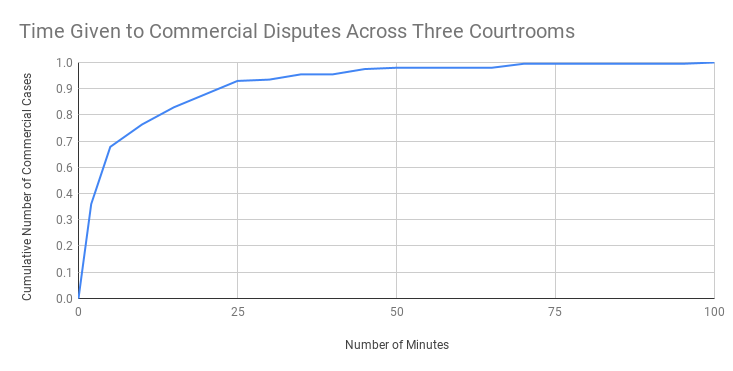
\includegraphics[height = 3in]{fig1.png}
\captionsetup{justification=centering}\caption[Optional Caption]{Cumulative Frequency Distribution of the Time Spent on Each Commercial Case Across Three Courtrooms in the 9-day Time-and-Motion Study}
\end{figure}

%Time Spent on Procedure, Substance and Adjournments
\subsubsection{Time Spent on Procedure, Substance and Adjournments}

The study found that, in general, less than 65\% of the total working hours of the court were spent on substantive matters and about 32\% on procedural matters and adjournments across the three courts, over the 9-day period (Table 3). \\

The provisions introduced by the Commercial Courts Act, 2015, streamlined various judicial tasks. Many procedural activities (e.g. recording evidence and witness statements) have now been brought under the purview of Judicial Registrars and Local Commissioners, thus saving the time of the Court. Despite that, in many cases, there was frequent back-and-forth between the parties and counsel over core issues, filing and evidence. This ended up requiring the discretion of the judge and, consequently, the time of the Court. Additionally, while the amendments to the Code of Civil Procedure by the Commercial Courts Act, 2015, direct judges to refuse adjournments for cases where the lawyers are absent, the research team observed several instances where adjournments were given in contravention of this directive. \\

In order to compare how the Court spent its time on commercial original-side cases as opposed to noncommercial original-side cases, the team calculated the proportion of the time spent on procedural, substantive matters and adjournments, specifically for commercial cases (Table 3).\\

%Table 3: Time Spent on Judicial Activities for Commercial and Noncommercial Original-Side Cases
\begin{table}[H]
\caption{Time Spent on Judicial Activities for Commercial and Non-Commercial Original Side Cases}
\footnotesize 
\begin{tabular}{L{3.5cm}C{3.5cm}C{3cm}C{3.5cm}}
\toprule
Type of Matters  & \multicolumn{3}{c}{Share of Time Spent Across 9 Days in Three Courtrooms (\%)} \\
\newline
& \textit{All Types of Cases}	&	\textit{Commercial Cases } 	& 	\textit{Noncommercial Cases}\\
\midrule
Procedural 	&  13.31  &  17.96  &   16.81 \\
Substantive 	&  64.28	&  71.60	& 49.00	\\
Adjournments &  19.24 & 10.43 &  34.19 \\
\bottomrule
\end{tabular}
\end{table}
\normalsize

Despite the fact that commercial cases were given less hearing time (Table 4) compared with noncommercial original-side disputes, the time-and-motion study found that commercial cases took lesser time on procedural matters and more time on substantive matters than noncommercial cases. The time spent on substantive stage for commercial disputes was 7.32 percentage points higher compared with all original-side cases.

%Do Commercial Cases Get the Dedicated Focus They Need?
\subsection{Do Commercial Cases Get the Dedicated Focus They Need?}
Given that the commercial bench does not look at commercial disputes exclusively, it is important to understand whether commercial disputes get the focus they require. This study attempted to approach this question by studying the relationship between time spent and pendency of commercial disputes as opposed to noncommercial original-side cases. It then went on to explore the proportion of time spent on commercial disputes in light of the time available to a judge per case.

%Is the Time Spent on Commercial Cases Proportional to Its Pendency?
\subsubsection{Is the Time Spent on Commercial Cases Proportional to Its Pendency?}
The team looked at the ratio of the pendency of cases which were commercial in nature to the other cases, which were filed before the original-side jurisdiction roster. The data for this were obtained from the \href{http://delhihighcourt.nic.in/instdisp.asp}{‘Real Time Pendency’ report} available on the website of the High Court of Delhi. 
The pendency as of 17 July 2018 was taken.\\

As of 17 July 2018, 41.43\% of all pending civil original-side cases at the High Court of Delhi were commercial cases (as defined by the Commercial Courts Act, 2015). Given the commercial bench has jurisdiction over both categories, this pendency proportion was compared to the time spent on commercial disputes in the time-and-motion study. The actual time spent on commercial original-side disputes, as opposed to noncommercial original-side disputes, was limited to 26.79\%. 
 
%Table 4:  Pendency and Time Allocated for Commercial and Noncommercial Original-Side Civil Cases in 2018
\begin{table}[H]
\caption{Pendency and Time Allocated for Commercial and Noncommercial Original Side Civil Cases in 2018}
\footnotesize
	\begin{tabular}{L{2.5cm}C{1.5cm}C{4cm}C{1.5cm}C{4cm}}
	\toprule
	Type of Case (Original Side) & \multicolumn{2}{L{5.5cm}}{Pending Cases (High Court of Delhi Real Time Pendency Report) (as of 17 July 2018)} & \multicolumn{2}{L{5.5cm}}{Time spent \newline(Time-and-Motion study) \newline(3 July-13 July 2018)}\\
\newline
	  & \textit{Number} & \textit{Proportion of total (\%)} & \textit{Minutes} & \textit{Proportion of total (\%)}\\
	  \midrule
	Commercial & 3664 & 41.43  & 1554.7 & 26.79\\
        	Noncommercial & 5180 & 58.57 & 4249 & 73.21\\
	\bottomrule
	\end{tabular}
\end{table}

%Time Available per Judge Versus Actual Time Spent on Commercial Cases
\subsubsection{Time Available per Judge Versus Actual Time Spent on Commercial Cases}
The data provided by the High Court of Delhi show that the number of judges on the bench has increased over the past 6 years. Simultaneously, the pendency for all original-side cases has gone down.\footnote{However, this could also be attributed to the change in pecuniary jurisdiction from Rs.20 lakh and above to Rs. 2 crore and above. A total of 10,886 cases were transferred from the High Court of Delhi to the District Courts as per the 2015–16 Annual Judiciary Report, along with 1,838 cases in 2016–17. These were not included in the final pendency statistics reported under Original-Side Cases in the Annual Judiciary Report.}  These data were used to perform a year-on-year comparison of the average time available per case per judge for all original-side cases. This was calculated as follows:\\

Average Time per Case per Judge\footnote{The formula for calculating average time per case per judge was taken from the biennial report published by the High Court of Delhi.} = 
\[\frac{300 \times{\textrm{Number of Judges}} \times {\textrm{Number of Working Days}}} {\textrm{Number of Cases}}\]

where 300 is the number of minutes in each working day.\footnote{From 10:30 am to 1:30 pm and then 2:30 pm to 5:30 pm.}\\

%\footnotetext{The formula for calculating average time per case per judge was taken from the biennial report published by the High Court of Delhi.}

Please note that the data for the years 2012–13 and 2014–15 is not publicly available, and thus the time available per bench per case for these time periods was not measured. Additionally, the pendency includes all cases listed under original jurisdiction for the High Court and does not differentiate commercial from noncommercial cases.\\

The time available per judge per case has increased progressively over the years for the original-side roster for the time period 2011–12, 2015–16, 2016–17 and 2018 (Table 5). 

%Table 5: Year-on-Year Comparison for Time Available per Bench per Case
\footnotesize
\begin{table} [H]
\caption[YoY Comparison for Time Available per Bench per Case]{YoY Comparison for Time Available per Bench per Case\footnotemark}
\begin{tabular}{L{4cm}C{2.2cm}C{2.2cm}C{2.2cm}C{2.2cm}}\\
\toprule
Parameter  & 2011- 2012 & 2015-2016 & 2016-2017 & 2018 \\
\midrule
Cases Pending & 15,782 & 10,768 & 9,218 & 8,844 \\
Judges in the Court & 6 & 6 & 5 & 7 \\
Judges in the Court & 6 & 6 & 5 & 7 \\
Annual Working Days & 211 & 211 & 215 & 221 \\
Daily Caseload per Judge & 12 & 8 & 9 & 6 \\
\midrule
Time available per Judge per Case (mins)* & 24 & 36 & 35 & 52 \\
\midrule
\multicolumn{5}{l}{\footnotesize{Sources: 2011-12: Biennial report of High Court of Delhi; 2015-16 and 2016-17: Supreme Court}}\\ 
\multicolumn{5}{l}{\footnotesize{of India Annual Report; 2018: Real Time Pendency Report High Court of Delhi. }}\\
\multicolumn{5}{l}{\footnotesize{*Numbers have been rounded up.}} \\
\bottomrule
\end{tabular}
\end{table}
\footnotetext{While the High Court publishes biennial report, it has not published this report after 2011-12. The data for 2018 was taken from the “Real Time Pendency” report published on the website of the High Court of Delhi (as of 17 July, 2018). The Supreme Court of India publishes an annual judiciary report which provided us with statistics for the High Court of Delhi. However, there was no report available for the remaining years on the website of Supreme Court of India.} 
\normalsize

%Will the New Approach Affect Disposal Times for Commercial Cases?
\subsection{Will the New Approach Affect Disposal Times for \\Commercial Cases?}

The Doing Business report of the World Bank estimates that it takes 1,445 days on average to resolve a contractual dispute in India. The study attempted to examine whether the constitution of the commercial bench at the High Court of Delhi would have an impact on the average time taken for the disposal of a commercial case. 

%Average Disposal Time for Commercial Cases
\subsubsection{Average Disposal Time for Commercial Cases}

To do this, the team first calculated the average time taken to dispose of a commercial original-side case (civil suit) in the High Court of Delhi in 2017. \\

There is no single repository of information on all commercial cases. This begs the question, how efficiently can one evaluate the performance of contract enforcement systems if they are not institutionally set up to monitor the results? \\

Disposal time could vary significantly for different kinds of civil disputes (e.g. a family dispute and dispute over licensing agreement), thus skewing averages for commercial disputes. Thus, using a measure of average disposal time for all cases would not be indicative of the performance of contract enforcement.

Therefore, the study team first created a database of commercial cases (civil suits) listed at the High Court of Delhi in the year 2017 (i.e. scheduled to be heard between 1 January 2017 and 31 December 2017), a total of 903 cases.\footnote{For the complete database, please refer to Annexures B and C; this is \href{http://bit.ly/2I7k8vH}{available online}.} Using the data, the team tried to understand the nature of disposal for all disposed-of cases and estimated the average time taken to resolve a commercial case. \\

The disposal time for settled and decreed cases was of specific interest because intuitively one might think that settlements took less than a full court hearing. On studying disposed commercial cases, the research team found that 37.97\% of the cases were decreed and 40\% of the cases were either withdrawn or settled (Figure 2). This finding was consistent with the results presented by Khaitan et al. \parencite{Vidhipaper}, wherein they argued that disposal rates could be skewed upwards due to cases which were withdrawn or settled early (compared with full hearings).

%Figure 2: Nature of Disposal 
\begin{figure}[H] %H means Here (HTPB = Here, Top, Page of Float, Bottom)
\centering
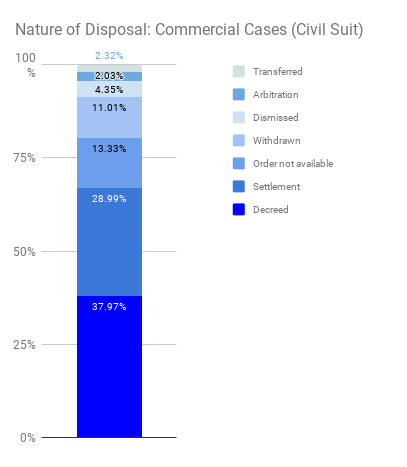
\includegraphics[height = 4.5in]{fig2.png}
\captionsetup{justification=centering}\caption[Optional Caption]{Nature of Disposal\footnotemark}
\end{figure}
\footnotetext{The nature of disposal includes the following activities: Decreed, judgement passed; Withdrawn, matter withdrawn by the party who initially filed the case; Settled, matter settled through mutual agreement between parties and no judgement passed; Transferred, matter transferred to another court; Dismissed, matter dismissed due to being of frivolous nature; Arbitration, matter settled through an arbitration process.}

Given the high mean disposal time for decreed cases, one might assume that full hearings took a long time for resolution. However, more outliers were observed within decreed cases, skewing the overall mean upwards. When the median disposal time was considered, the average was actually lower for decreed cases. At a closer examination, the study found that more than 80\% of the decreed and settled cases had similar disposal time, thus indicating little difference between the two (Figure 3). 

%Figure 3: Average Disposal Time Decreed Versus Settled Cases 
\begin{figure}[H] %H means Here (HTPB = Here, Top, Page of Float, Bottom)
\centering
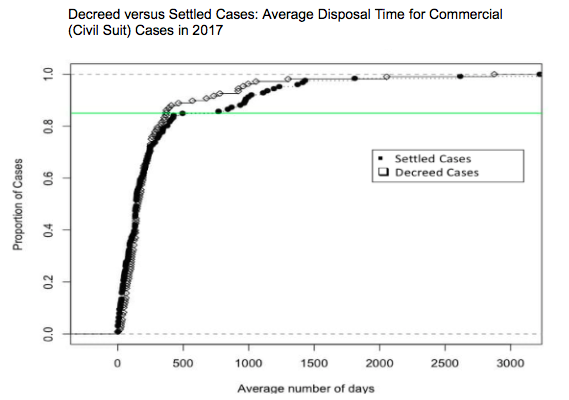
\includegraphics[height = 3.7in]{fig3.png}
\captionsetup{justification=centering}\caption[Optional Caption]{Average Disposal Time Decreed Versus Settled Cases}
\end{figure}

When the team studied the days between filing and disposal for commercial cases, the median disposal time was surprisingly low compared with the World Bank estimates. Compared with the figures put out by the bank, it appeared that, for the January 2017 to December 2017 period, in the High Court of Delhi, the median time for disposal for commercial original-side cases (civil suits) was only about 151 days (Table 6). Additionally, the average time taken between hearings was 39 days. 

%Table 6: Average Disposal Time (in Days)
\begin{table}[H]
\caption{Average Disposal Time (in Days)}
	\begin{tabular}{L{4cm}C{3cm}C{3cm}C{3cm}}
	\toprule
	& \multicolumn{3}{c}{Days Between Filing and Disposal}\\
	  & \footnotesize{\textit{Disposed (All)}} & \footnotesize{\textit{Decreed}} & \footnotesize{\textit{Settled}}\\
	\midrule
	\normalsize
	{Mean} & 448 & 639 & 273\\
	{Median} & 151 & 142 & 154\\
	{Max} &  40865 &40865 & 2876\\
	 \bottomrule
	\end{tabular}
\end{table}

It is important to view these results in light of the existing pendency. Commercial courts were proposed to ‘speed things up’; however, in this case, no specialised court was actually set up. To increase judicial efficiency, the time allotted to commercial disputes, especially in the substantive stage, will need to increase.  

%================CONCLUSION======================================================
\section*{Conclusion}
\addcontentsline{toc}{section}{Conclusion}

The Commercial Courts Act, 2015, introduced the provision to set up commercial courts at District and High Court levels. Following the Act, the High Court of Delhi instituted a commercial division. \\

When the team visited the commercial division at the High Court of Delhi, their first observation was the lack of an exclusive commercial division. It was also found that commercial disputes did not have any time slots dedicated exclusively for them at the High Court of Delhi. There was no distinction in the way commercial cases and ordinary civil disputes were handled by the judge. Commercial cases were listed along with other civil original-side disputes and were heard and proceeded the same way. In fact, other civil disputes were given more of the division’s time. \\

While the time available to a judge in the commercial division (per case) has increased over the years, the time spent on commercial disputes was not found to be proportional to relative pendency or to time available with the judge when comparing pendency of commercial disputes to all original-side cases. \\

Additionally, the study found that the median disposal time for commercial cases in 2017 was surprisingly low compared with the World Bank estimates. Achieving further efficiency gains will likely require a substantial increase in the amount of time dedicated towards commercial disputes.\\

This study only examined commercial original-side cases (civil suit) for a short period of time. Consequently, how this maps out for appeals and lower courts is unclear. Despite this caveat, the nonspecialised approach will likely not take us quite far in improving judicial efficiency at the High Court level. \\

Systems adopted in other countries may offer some clues to bring about further efficiency gains. In the case of Ireland, the case management system is such that core issues, evidence and witness statements are agreed upon beforehand, avoiding back-and-forth during the trial. In Uganda, courts were exclusively set up for commercial disputes with dedicated judges and frequent training in the dynamic realm of commerce \parencite{ugandapaper}. Positive gains were observed in England with such specialisation, where mean disposal time (filing to hearing) reduced by 57.2\% from 2006 to 2015 \parencite{MOJUKreport}. In particular, the study suggested that the government worked on reforms which reduced the time spent by judges on procedural matters and adjournments. \\

While this study attempted to understand the current state of commercial courts in Delhi and discern potential areas of improvement, it did not address causality or try to determine which model would work best for India. Further research would be needed to arrive at an appropriate model.\\

On a final note, the EoDB ranking parameter for contract enforcement considers cases whose claim size would amount to be Rs. 321,665 or above for India. The Commercial Courts Act, 2015, only affected cases with a listed claim amount of Rs. 1 crore or above. With the Commercial Courts Amendment Act, 2018, this claim value has been brought down to Rs. 300,000, thus including all cases which would be evaluated to determine the Contract Enforcement Rank of India. If India is able to achieve improved efficiency within specialised commercial courts (i.e. reduce time and costs for such cases), it can possibly impact our EoDB ranking.

%================BIBLIOGRAPHY=====================================================
\newpage
\section*{Bibliography}
\addcontentsline{toc}{section}{Bibliography}
\printbibliography[heading=none] 

%================APPENDICES=====================================================
%Appendix 1
\newpage      
\section*{Appendix 1: Day-Wise Breakdown of Time and \\ Motion Study across three courtrooms}
\addcontentsline{toc}{section}{Appendix 1: Day-Wise Breakdown of Time and \\ Motion Study across three courtrooms}
%Table 7: Day-Wise Breakdown of Time and Motion Study across Three Courtrooms
\footnotesize
\begin{longtable}[l]{>{\raggedright}p{3.8cm}>{\raggedleft}p{1cm}>{\raggedleft}p{1cm}>{\raggedleft}p{1cm}>{\raggedleft}p{1cm}>{\raggedleft}p{1cm}>{\raggedleft\arraybackslash}p{1cm}}
  \caption{Day-Wise Breakdown of Time and Motion Study across Three Courtrooms}\\
\toprule
\multicolumn{7}{c}{A = Time (hh:mm:ss); B = Percentage share of the day} \\
\midrule
          &	A 	& 	B 	  &	A 	& 	B 	  &	A 	& 	B\\ 	 
& \multicolumn{2}{c}{\textit{\textbf{Courtroom \#19}}} & \multicolumn{2}{c}{\textit{\textbf{Courtroom \#20}}} & \multicolumn{2}{c}{\textit{\textbf{Courtroom \#23}}} \\
\midrule
\endfirsthead
\toprule
\multicolumn{7}{c}{A = Time (hh:mm:ss); B = Percentage share of the day} \\
\midrule
          &	A 	& 	B 	  &	A 	& 	B 	  &	A 	& 	B\\ 	 
& \multicolumn{2}{c}{\textit{\textbf{Courtroom \#19}}} & \multicolumn{2}{c}{\textit{\textbf{Courtroom \#20}}} & \multicolumn{2}{c}{\textit{\textbf{Courtroom \#23}}} \\
\midrule
\endhead
\endfoot
\endlastfoot
    \multicolumn{7}{c}{Day 1: 03-Jul-18} \\
    \midrule
    Court in Session & 2:28:00 &       & 3:54:15 &       & 2:36:15 &  \\
    Procedural matters & 0:13:00 & 8.78  & 0:17:44 & 7.57  & 0:05:24 & 3.46 \\
    Adjournments matters & 0:00:00 & 0     & 0:55:00 & 23.48 & 0:11:18 & 7.23 \\
    Substantive matters & 2:15:00 & 91.22 & 2:32:15 & 64.99 & 2:12:36 & 84.86 \\
    \midrule
    \multicolumn{7}{c}{Day 2: 04-Jul-18} \\
    \midrule
    Court in session & 2:55:00 &       & 4:05:47 &       & 2:47:55 &  \\
    Procedural matters & 0:19:00 & 10.9  & 0:23:07 & 9.4   & 0:55:06 & 32.8 \\
    Adjournments matters & 0:10:00 & 5.7   & 0:33:58 & 13.8  & 0:50:07 & 29.9 \\
    Substantive matters & 2:25:00 & 82.9  & 2:59:18 & 72.9  & 0:44:57 & 26.8 \\
    \midrule
    \multicolumn{7}{c}{Day 3: 05-Jul-18} \\
    \midrule
    Court in session & 2:57:00 &       & 4:51:01 &       & 2:53:01 &  \\
Procedural matters & 0:16:00 & 9     & 1:34:12 & 32.4  & 0:24:51 & 14.4 \\
    Adjournments matters & 0:09:00 & 5.1   & 0:31:54 & 10.9  & 0:31:28 & 18.2 \\
    Substantive matters & 2:32:00 & 85.9  & 2:27:50 & 50.9  & 1:49:39 & 63.4 \\
    \midrule
    \multicolumn{7}{c}{Day 4: 06-Jul-18} \\
    \midrule
Court in session & 2:35:00 &       & 4:21:22 &       & 3:42:57 &  \\
Procedural matters & 0:21:00 & 13.6  & 0:23:47 & 9.1   & 0:29:50 & 13.4 \\
Adjournments matters & 0:08:00 & 5.2   & 1:44:22 & 39.9  & 0:47:46 & 21.4 \\
Substantive matters & 2:06:00 & 81.3  & 2:00:08 & 45.9  & 2:13:22 & 59.8 \\
   \midrule
    \multicolumn{7}{c}{Day 5: 09-Jul-18} \\
    \midrule
Court in session & 0:45:00 &       & 5:09:39 &       & 2:57:45 &  \\
Procedural matters & 0:26:30 & 58.9  & 0:31:51 & 10.3  & 1:36:12 & 54.1 \\
Adjournments matters & 0:12:00 & 26.7  & 0:46:36 & 15.1  & 0:25:39 & 14.4 \\
Substantive matters & 0:06:30 & 14.4  & 3:35:47 & 69.7  & 0:20:21 & 11.5 \\
\midrule
    \multicolumn{7}{c}{Day 6: 10-Jul-18} \\
    \midrule
Court in session & 3:02:00 &       & 4:58:06 &       & 3:25:23 &  \\
Procedural matters & 0:41:30 & 22.8  & 0:43:34 & 14.6  & 1:25:37 & 41.7 \\
Adjournments matters & 0:03:00 & 1.7   & 0:51:03 & 17.1  & 0:38:12 & 18.6 \\
Substantive matters & 2:17:30 & 75.6  & 3:17:55 & 66.4  & 0:59:00 & 28.7 \\
\midrule
    \multicolumn{7}{c}{Day 7: 11-Jul-18} \\
    \midrule
Court in session & 3:27:00 &       & 4:43:07 &       & 2:59:18 &  \\
Procedural matters & 0:18:00 & 8.7   & 0:35:56 & 12.7  & 1:08:16 & 38.1 \\
Adjournments matters & 0:01:00 & 0.5   & 0:31:03 & 10.9  & 0:14:19 & 7.9 \\
Substantive matters & 3:08:00 & 90.8  & 3:24:38 & 72.3  & 1:25:04 & 47.5 \\
\midrule
    \multicolumn{7}{c}{Day 8: 12-Jul-18} \\
    \midrule
Court in session & 3:45:30 &       & 4:47:32 &       & 3:53:35 &  \\
Procedural matters & 0:11:30 & 5.1   & 0:17:08 & 5.9   & 0:28:09 & 12.1 \\
Adjournments matters & 0:07:00 & 3.1   & 0:30:38 & 10.7  & 0:16:37 & 7.1 \\
Substantive matters & 3:27:00 & 91.8  & 3:54:52 & 81.7  & 2:59:38 & 76.9 \\
\midrule
    \multicolumn{7}{c}{Day 9: 13-Jul-18} \\
    \midrule
Court in session & 3:46:00 &       & 4:58:02 &       & 3:58:13 &  \\
Procedural matters & 0:54:30 & 24.1  & 0:57:16 & 19.2  & 1:03:03 & 26.5 \\
Adjournments matters & 0:22:00 & 9.7   & 0:33:21 & 11.2  & 0:56:45 & 23.8 \\
Substantive matters & 2:29:30 & 66.2  & 3:01:02 & 60.7  & 2:48:37 & 70.8 \\
    \bottomrule      
\end{longtable}
\normalsize 

\footnotesize
\begin{longtable}[l]
{>{\raggedright}p{3.3cm}>{\raggedright}p{3cm}>{\raggedright}p{3cm}>{\raggedright\arraybackslash}p{3cm}}\\
\toprule
    {\textbf{Average}} & \textit{\textbf{Courtroom \#19}} & \textit{\textbf{Courtroom \#20}} & \textit{\textbf{Courtroom \#23}} \\
\midrule
    Time court was in session & 2:51:10 & 4:38:46 & 3:14:56 \\
\midrule
\multicolumn{4}{c}{Proportion of Time Spent}\\
\midrule
    Procedural matters & 17.98\% & 13.47\% & 26.27\% \\
    Adjournment matters & 6.40\% & 17.02\% & 16.52\% \\
    Substantive matters & 75.56\% & 65.05\% & 52.24\% \\
\bottomrule
\end{longtable}%
\normalsize

\end{document}
